\chapter{Multi-view recalibration}
\label{cha:multi-view calibration}

The connexion between the previous defined components will be provided here, explaining the way they are working together in both the acquisition and estimation process. Recall the goal is to recalibration multiples cameras, using the PR2 as a real example, but focused in the estimation part.

\section{Preliminary}

\subsection{Camera model in ROS}

* Camera model (in the ROS context)
* Rect Images (no distortion)

* Type of messages
*

\subsection{PR2 cameras}

The camera configuration can be seen in Figure \ref{fig:pr2_cameras}.
The PR2 has 6 cameras in its head:
\begin{itemize*}
 \item 2 narrow range. Topics: \texttt{wide\_right\_rect} and \texttt{wide\_left\_rect}.
 \item 2 wide range. Topics: \texttt{narrow\_right\_rect} and \texttt{narrow\_left\_rect}.
 \item 1 Kinect. Topic: \texttt{kinect\_head}.
 \item 1 High definition. Topic: \texttt{Prosilica\_rect}.
\end{itemize*}

\begin{figure}[!htbp]
 \centering
 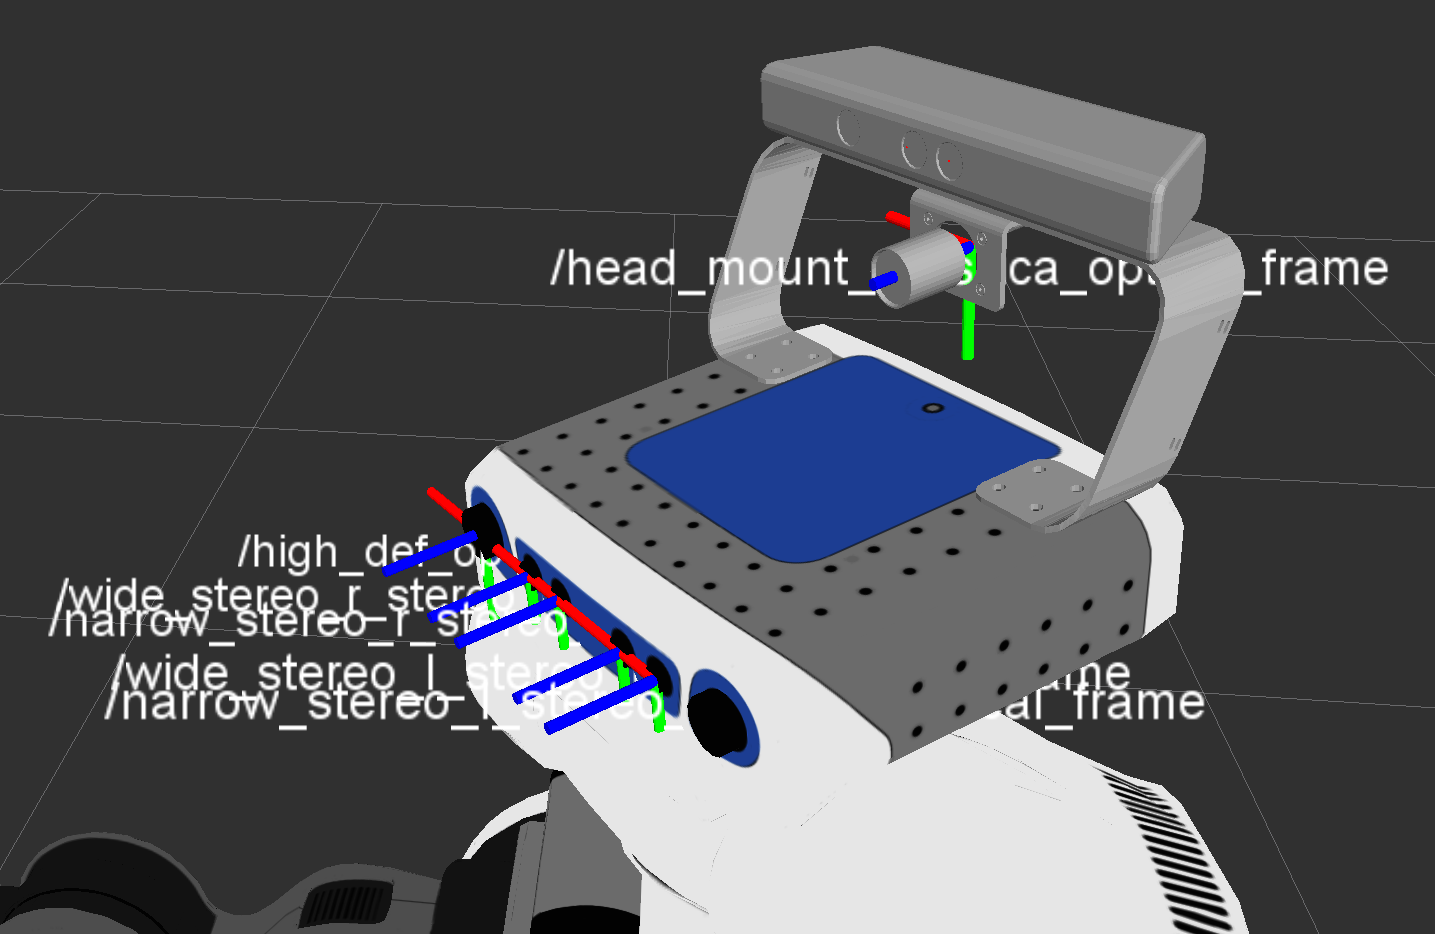
\includegraphics[width=0.75\textwidth]{images/screenshots/PR2_cameras.png}
 \caption{Coordinate system of all the cameras in the PR2 head.}
 \label{fig:pr2_cameras}
\end{figure}






\section{Acquisition process}
\label{sec:acquisition}

The acquisition part was already implemented, and a full description can be found in the paper  \cite{pr2_calibration_paper} and in the ROS tutorials for the PR2 calibration package.

% The thesis is focused in the estimation part but, in order to reach part, it is necessary first to do some comments regarding the process and
%
% % In the paper  and the ROS tutorials for the PR2 calibration package, the full description of the acquisition process will
% In this section will explain the acquisition process. It will explain


\subsection{Data collection}

In order to sufficiently constrain the non-linear optimization (see \cite{pr2_calibration_paper}), it is needed to collect a large amount of data, and manually collecting this calibration data can be tedious. By having the PR2 hold a checkerboard in its gripper (Figure~\ref{fig:pr2_holdind_cb}), a total of 30 checkerboard poses measurements are collected for each hand. Also, 4 samples of a large checkerboard that is far from the robot in order to help with far-field calibration. This data is saved in a ROS bag (section~\ref{sec:rosbag}) and posteriorly processed for the calibration package.

\begin{figure}[!htbp]
 \centering
 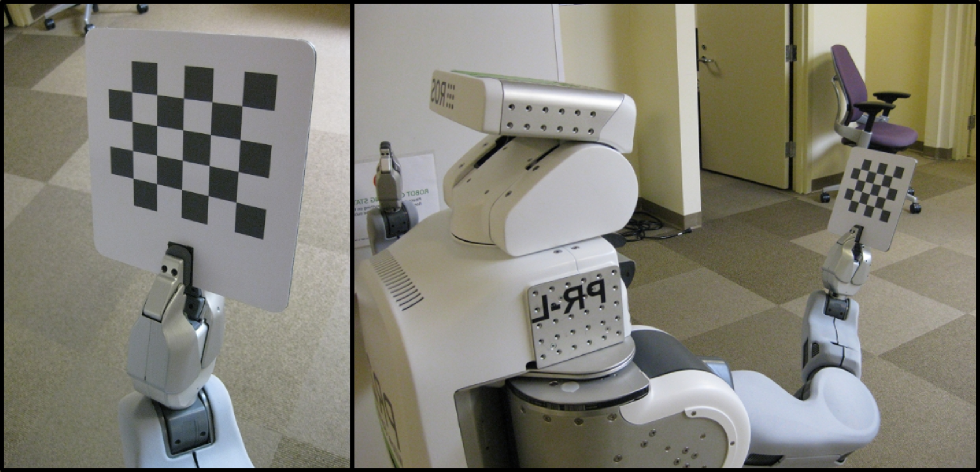
\includegraphics[width=0.5\textwidth]{images/pr2_holdind_cb.png}
 \caption{The PR2 holding a checkerboard pattern.}
 \label{fig:pr2_holdind_cb}
\end{figure}


